\section{Personas}\label{sec:persona}

Personas erhalten ihren Namen von den gleichnamigen Masken antiker Schauspieler.
Entwickelt wurden sie Ende der 90er Jahre von Alan Cooper \cite{PersonaCooper}.
Personas sind fiktive Personen, welche die durchschnittlichen Nutzenden widerspiegeln sollen.
Eine Persona ist somit nie von einer konkreten Person inspiriert, mehr von einer Gruppe an Personen.
Im Normalfall werden im Zuge des nutzungsorientierten Prozesses einige wenige Personas erstellt, welche zusammen einen möglichst großen Teil der Nutzenden abdeckt.

Personas ermöglichen es den Entwickelnden für konkrete Personen zu entwickeln.
Dies ist hilfreich, wenn über die Umsetzung eines Features diskutiert wird.
Hier kann überlegt werden, ob die Persona dieses Feature hilfreich findet.
Das Argument "Irgendjemand will doch sicher..." ist somit hinfällig.
Es ist auch möglich, eine Persona zu erstellen, welche das Gegenteil der Nutzenden verkörpert und gegen welche das System ausgerichtet wird.

\begin{figure}[htp]
    \centering
    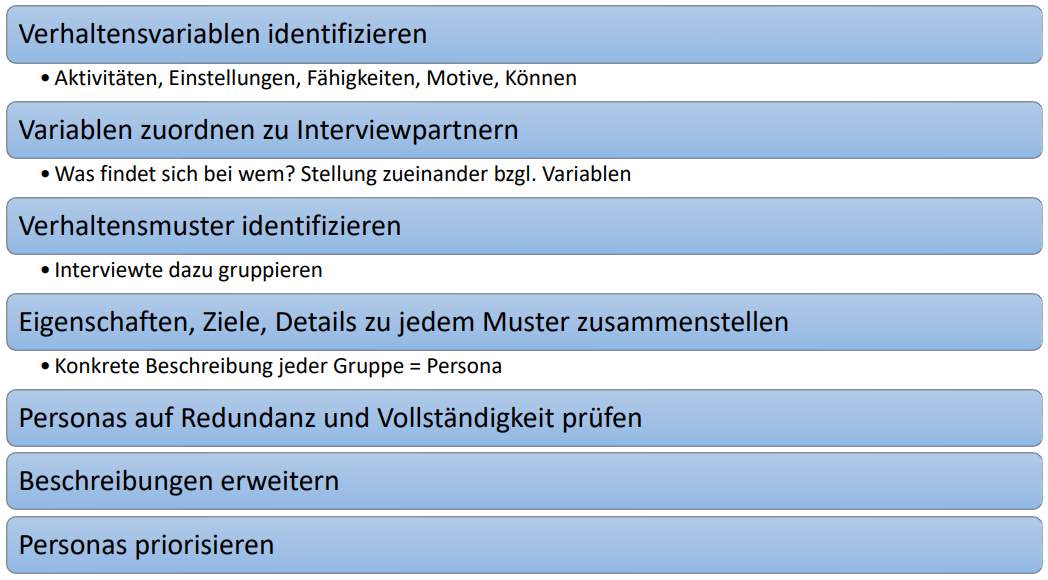
\includegraphics[width=\textwidth]{images/Persona-Leitfaden.png}
    \caption{Leitfaden zum Erstellen von Personas}
    \label{fig:personaLeitfaden}
\end{figure}

Da Personas Nutzende verallgemeinern ist zu beachten, dass hier häufig Stereotypen entstehen.
Bei der Erstellung ist es somit wichtig, nicht auf Vorurteile zurück zufallen.
Sollten mehrere Personas entwickelt werden, so ist zu beachten, dass diese eine möglichst kleine Überschneidung in ihren Merkmalen haben sollen.
Ziel ist es, auf effiziente Weise mit so wenig Personas wie möglich einen möglichst großen Raum der Nutzenden abzudecken.

Personas sollen erlebbar sein.
Hierzu ist es wichtig, diese auch über die für den Kontext wichtigen Attribute zu entwerfen.
Personas haben praktische und persönliche Ziele, betreiben bestimmte Aktivitäten, haben Hobbys und Einstellungen, sowie personalisierte Fähigkeiten, Wissen und Erfahrungen.
Ebenso soll ihre Herkunft, Bildung, Aussehen und ihre Familienbeziehung klar aus der Beschreibung hervor gehen.

Personas werden aus empirischen Erhebungen erstellt.
Hierzu kann einem Leitfaden gefolgt werden.
Dieser ist von Cooper, Reimann und Cronin \cite{PersonaCooperEtA} entwickelt worden und in \autoref{fig:personaLeitfaden} zu sehen\footnote{Konzept von Cooper, Reimann und Cronin aus \cite{PersonaCooperEtA}, Darstellung aus \cite{NOG}}.

Die Darstellung einer Persona kann unterschiedlich sein.
Sie kann auf Papier gezeichnet werden, in einem Text beschrieben werden oder auch grafisch dargestellt werden.
Einige Beispiele von Personas sind im Anhang unter \autoref{ap:personas} zu finden. 
Darüber hinaus ist in \autoref{fig:personaPaul} eine Persona für den hier praktisch behandelten Kontext zu finden.